\section{Setup}
\frame{\tableofcontents[currentsection, hideothersubsections]}

\begin{frame}
\frametitle{Experiment Setup}

\begin{itemize}
  \item 20 simulated physics task,
  including classic problems such as cartpole swing-up, dexterous manipulation, legged locomotion and car driving
  \item non-linear fn approx
  \item a baseline computed by a planner (Tassa et al., 2012) that
  has full access to the underlying simulated dynamics and its derivatives (see supplementary information).
  \item ran experiments using both a low-dimensional state description (such as joint angles and positions) and high-dimensional renderings of the environment
\end{itemize}

\end{frame}


\begin{frame}
\frametitle{Assumptions, Baselin}

Assumption:
\begin{itemize}
  \item env is MDP, the environment is fully-observed
\end{itemize}


Baseline:
\begin{itemize}
  \item the mean return from a naive policy which samples actions from
  a uniform distribution over the valid action space
  \item iLQG, a planning based solver with full access to
  the underlying physical model and its derivatives.
\end{itemize}

\end{frame}

\begin{frame}
\frametitle{Tasks}
\begin{figure}
    \centering
    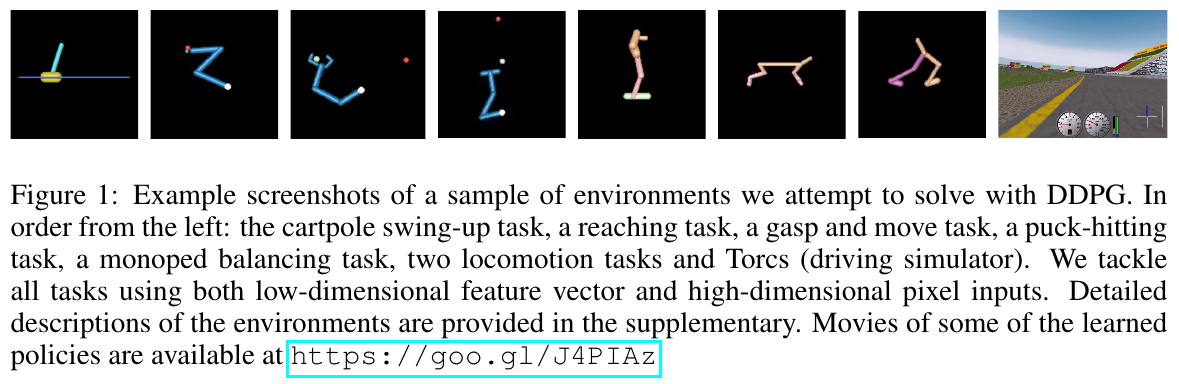
\includegraphics[scale=0.3]{fig_1}
\end{figure}
\end{frame}
